\documentclass{article}

\usepackage{url}
\usepackage{graphicx}	% For figure environment
\usepackage{epstopdf}
\usepackage[center]{subfigure}
\usepackage{amssymb}	% For mathematical figures like \mathbb{R}
\usepackage{amsmath}
\usepackage{framed}

\title{Advanced Systems Lab - Milestone I} 
\author{Lukas Elmer, Matthias Ganz} 
\date{\today} 


\begin{document}

\maketitle


\begin{abstract}

This document, describes the message queuing system which was build. Architecture and design choices are shown and explained. Further test scenarios and test loads are defined. Resulting test output is described and analysed.

\end{abstract}

%% %%%%%%%%%%%%%%%%%%%%%%%%%%%%%%%%%%%%%%%%%%%%%%
\section{Messaging System}
In this section the system under test (or middle ware component) is described.


%% ----------------------------------------------
\subsection{Overview}

\begin{figure}
  \begin{center}
    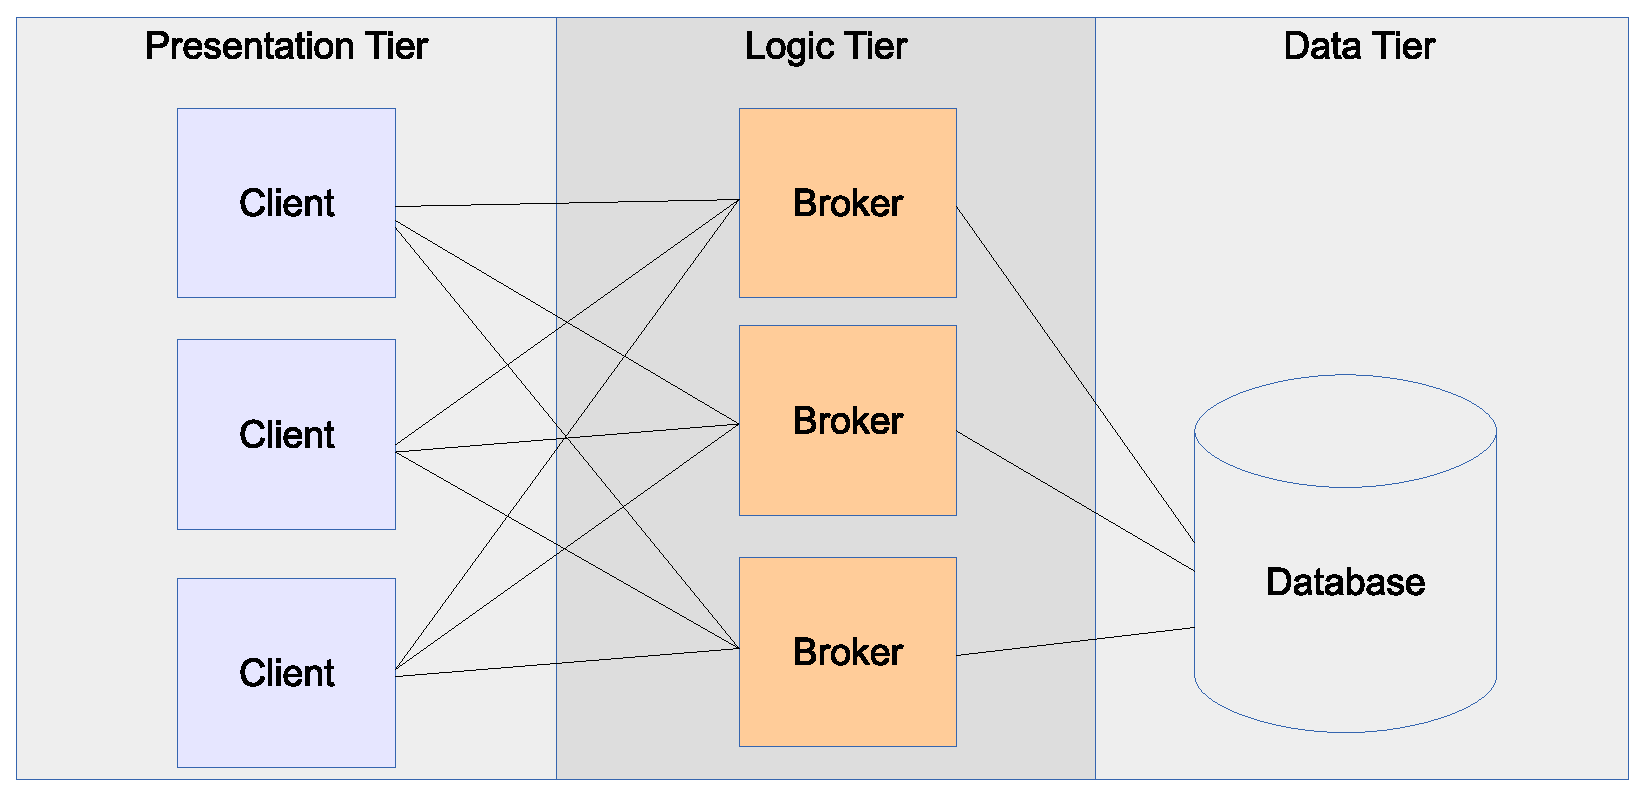
\includegraphics[scale=0.4]{../drawings/system-overview.eps}
  \end{center}
  \caption{System Overview}
  \label{fig:system-overview}
\end{figure}


%% ----------------------------------------------
\section{Messaging System}

\begin{figure}
	\begin{center}
    \includegraphics[scale=0.4]{../drawings/broker-threading.eps}
  \end{center}
  \caption{Middleware's main Components}
  \label{fig:middleware-threading}
\end{figure}

%% ----------------------------------------------
\section{Design Decisions}

\subsection{Schead Load}
Schead load
blocking reqeust response queues suboptimal

If queue full, immediately stop request

\subsection{NIO vs IO}

NIO VS Blocking IO

\subsection{Connection Pooling}

\subsection{Buffer Pooling}


\subsection{Message Transmission}


%% %%%%%%%%%%%%%%%%%%%%%%%%%%%%%%%%%%%%%%%%%%%%%%%%%%%%%%%%%%%%%%%%%%%%%%%%%
\section{How We Measured Our System}

\subsection{Hypothesis}

%% %%%%%%%%%%%%%%%%%%%%%%%%%%%%%%%%%%%%%%%%%%%%%%%%%%%%%%%%%%%%%%%%%%%%%%%%%
\section{Notes - to delete}

\subsection{What should be included in this report }

\subsubsection{System Code}
\begin{itemize}
\item Code
\item Scripts for experiment
\end{itemize}

\subsubsection{Experimental data}
\begin{itemize}
\item Basic tests ans simple traces
\item Long running traces, Raw data and graphs for all experiments
\end{itemize}

\subsubsection{Written report}
\begin{itemize}
\item Architectural  diagrams
\item Interface description
\item explanation of the system design
\item Description of all experiments
\item statistical treatment of data
\item commentary analysis
\end{itemize}



\end{document}
